\documentclass[12pt]{article}

\usepackage{amsmath}


\usepackage[utf8]{inputenc}
\usepackage[T1, T2A]{fontenc}
\usepackage{fullpage}
\usepackage{multicol, multirow}
\usepackage{tabularx}
\usepackage{ulem}
\usepackage{listings}
\usepackage[english, russian]{babel}
\usepackage{tikz}
\usepackage{pgfplots}
\usepackage{indentfirst}
\usepackage{noindentafter}
\usepackage{nonfloat}
\usepackage{ulem}
\usepackage{fancyhdr}
% \usepackage{courier}
% \usepackage{FiraMono}
\usepackage{color}
\usepackage{subcaption}
\usepackage{titlesec}


\parindent=1cm

\linespread{1}
\pgfplotsset{compat=1.16}
\newcommand{\se}[1]{\section*{\bf #1}}

\newcommand{\listsource}[2]{
	\subsection*{\textbf{#2}}
	{\footnotesize
		\lstinputlisting[language=c++]{#1/#2}
	}
}

\lstdefinestyle{empty}{language=c++,
	basicstyle=\scriptsize,
	showspaces=false,
	showstringspaces=false,
	showtabs=false, вариантов
	tabsize=4,
	breaklines=true,
	escapechar=@,
	numbers=none,
	frame=none,
	escapeinside={\%*}{*)},
	breakatwhitespace=false % переносить строки только если есть пробел
}

\lstdefinestyle{customc}{
	belowcaptionskip=1\baselineskip,
	breaklines=true,
	frame=L,
	xleftmargin=\parindent,
	language=c++,
	numbers=left,
	showstringspaces=false,
	basicstyle=\footnotesize\ttfamily,
	keywordstyle=\bfseries\color{green!40!black},
	commentstyle=\itshape\color{purple!40!black},
	identifierstyle=\color{blue},
	stringstyle=\color{orange},
}

\lstset{escapechar=@,style=customc}

\pgfplotsset{compat=1.17}

\titleformat{\section}
{\normalfont\Large\bfseries}{\thesection.}{0.3em}{}

\titleformat{\subsection}
{\normalfont\large\bfseries}{\thesubsection.}{0.3em}{}

% \titlespacing{\section}{0pt}{*2}{*2}
% \titlespacing{\subsection}{0pt}{*1}{*1}
% \titlespacing{\subsubsection}{0pt}{*0}{*0}
% \lstloadlanguages{Lisp}
% \lstset{extendedchars=false,
% 	escapechar= |,
% 	breaklines=true,
% 	breakatwhitespace=true,
% 	keepspaces = true,
% 	tabsize=2
% }

\newcommand{\makemytitlepage}[2]{
	\thispagestyle{empty}
	\begin{center}
		\bfseries

		{\Large Московский авиационный институт\\ (национальный исследовательский университет)

		}

		\vspace{48pt}

		{\large
			Институт №8 ``Информационные технологии и прикладная математика''
			Кафедра 806 ``Вычислительная математика и программирование''
		}

		\vspace{36pt}

		{Лабораторная работа №#1  \\
			По курсу ``Программирование графических процессоров''
		}
		\vspace{48pt}

		{#2}

	\end{center}

	\vspace{72pt}

	\begin{flushright}
		\begin{tabular}{rl}
			Выполнил:      & П.\, А. Милько      \\
			Группа:        & М8О-408Б-17         \\
			Преподаватели: & К.Г. Крашенинников, \\
			               & А.Ю. Морозов.       \\
		\end{tabular}
	\end{flushright}

	\vfill

	\begin{center}
		\bfseries
		Москва\\
		\the\year
	\end{center}
	\newpage
	\setcounter{page}{1}
}

\newcommand{\nvidia}[0]{
	\se{Программное и аппаратное обеспечение}
	
	TODO
}
\renewcommand{\cource}{Параллельная обработка данных}

\newcommand{\makemytitlepagee}[1]{
        \thispagestyle{empty}
        \begin{center}
                \bfseries

                {\Large Московский авиационный институт\\ (национальный исследовательский университет)

                }

                \vspace{48pt}

                {\large
                        Институт №8 ``Информационные технологии и прикладная математика''
                        Кафедра 806 ``Вычислительная математика и программирование''
                }

                \vspace{36pt}

                \vspace{48pt}

                {#1}

        \end{center}

        \vspace{72pt}

        \begin{flushright}
                \begin{tabular}{rl}
                        Выполнил:      & П.\, А. Милько      \\
                        Группа:        & М8О-408Б-17         \\
                        Преподаватели: & К.Г. Крашенинников, \\
                                       & А.Ю. Морозов.       \\
                \end{tabular}
        \end{flushright}

        \vfill

        \begin{center}
                \bfseries
                Москва\\
                \the\year
        \end{center}
        \newpage
        \setcounter{page}{1}
}

\begin{document}
\makemytitlepagee{Обратная трассировка лучей (Ray Tracing) на GPU}

\se{Цель работы}
Использование GPU для создание фотореалистической визуализации.
Рендеринг полузеркальных и полупрозрачных правильных геометрических тел.
Получение эффекта бесконечности. Создание видеоролика.



\textbf{Сцена}

Прямоугольная текстурированная поверхность (пол), над которой
расположены три платоновых тела. Сверху находятся несколько источников света. На
каждом ребре многогранника располагается определенное количество точечных
источников света. Грани тел обладают зеркальным и прозрачным эффектом. За счет
многократного переотражения лучей внутри тела, возникает эффект бесконечности.

\textbf{Камера}

Камера выполняет облет сцены согласно определенным законам. В
цилиндрических координатах $(r,\varphi,z)$, положение и точка направления камеры в
момент времени $t$ определяется следующим образом:

\begin{equation*}
	\begin{split}
		r_c(t) &=r_c^0+A_c^r \sin(\omega_c^r\cdot t + p_c^r) \\
		z_c(t) &=z_c^0+A_c^z \sin(\omega_c^z\cdot t + p_c^z) \\
		\varphi_c(t) &= \varphi_c^0 +\omega_c^\varphi \cdot t \\
		r_n(t) &=r_n^0+A_n^r \sin(\omega_n^r\cdot t + p_n^r) \\
		z_n(t) &=z_n^0+A_n^z \sin(\omega_n^z\cdot t + p_n^z) \\
		\varphi_n(t) &= \varphi_n^0 +\omega_n^\varphi \cdot t \\
	\end{split}
\end{equation*}

\textbf{Задание}

Требуется реализовать алгоритм обратной трассировки лучей с использованием технологии CUDA.
Выполнить покадровый рендеринг сцены. Для устранения эффекта ``зубчатости'',
выполнить сглаживание (например с помощью алгоритма SSAA).
Полученный набор кадров склеить в видеоролик любым доступным программным обеспечением.
Подобрать параметры сцены, камеры и освещения таким образом, чтобы получить наиболее красочный результат.
Провести сравнение производительности gpu и cpu (т.е. дополнительно нужно реализовать алгоритм без использования CUDA).

Согласно варианту 10 на сцене должны располагаться три тела: Октаэдр, Додекаэдр, Икосаэдр.

\textbf{Входные данные.}

Программа должна принимать на вход следующие параметры:

\begin{enumerate}
	\item Количество кадров.

	\item Путь к выходным изображениям. В строке содержится спецификатор \%d, на
	      место которого должен подставляться номер кадра. Формат изображений
	      соответствует формату описанному в лабораторной работе 2.

	\item Разрешение кадра и угол обзора в градусах по горизонтали.

	\item Параметры движения камеры \\
	      $r_c^0, z_c^0, \varphi_c^0, A_c^r, A_c^z, \omega_c^r, \omega_c^z, \omega_c^\varphi, p_c^r$ и \\
	      $r_n^0, z_n^0, \varphi_n^0, A_n^r,A_n^z,\omega_n^r,\omega_n^\varphi, p_n^r, p_n^z$.

	\item Параметры тел:
	      центр тела,
	      цвет (нормированный),
	      радиус (подразумевается радиус сферы в которую можно было бы вписать тело),
	      коэффициент отражения,
	      коэффициент прозрачности,
	      количество точечных источников света на ребре.

	\item Параметры пола: четыре точки, путь к текстуре, оттенок цвета и коэффициент отражения.

	\item Количество (не более четырех) и параметры источников света: положение и цвет.

	\item Максимальная глубина рекурсии и квадратный корень из количества лучей на один пиксель (для SSAA).
\end{enumerate}

\noindent Программа должна поддерживать следующие ключи запуска:

\begin{itemize}
	\item \lstinline@--cpu@ для расчетов используется только центральный процессор.
	\item \lstinline@--gpu@ для расчетов задействуется видеокарта.
	\item \lstinline@--default@
	      В stdout выводится конфигурация входных данных (в формате
	      описанном ранее) при которой получается наиболее красочный результат, после чего
	      программа завершает свою работу.
\end{itemize}

Запуск программы без аргументов подразумевает запуск с ключом --gpu.
В процессе работы программа должна выводить в stdout статистику в формате:

\nvidia

\se{Метод решения}

Так как нужно использовать mpi, то логично разделить вычисления по рендеру кадров.
Код в варианте для CPU использует OpenMP чтобы сильно не отставать от GPU и оптимально
использовать ресурсы процессора.

Для варианта на CUDA пиксели обрабатываются в блоках небольшого размера (16x16),
а для cpu проход по пикселям линейный и за счёт этого прекрасно параллелится с помощью директивы \lstinline|omp parallel for|.

Для сглаживания использовался алгоритм SSAA как самый простой в реализации.
Хотя он довольно сильно ударил по производительности.

\se{Исходный код}

\listsource{../src/render}{render.cu}
\listsource{../src/render}{render.cpp}

\se{Результаты}

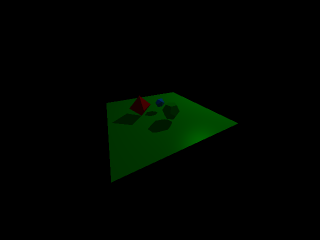
\includegraphics{small.png}

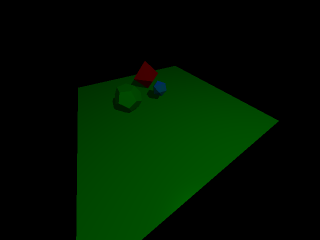
\includegraphics{small_2.png}

\smallbreak

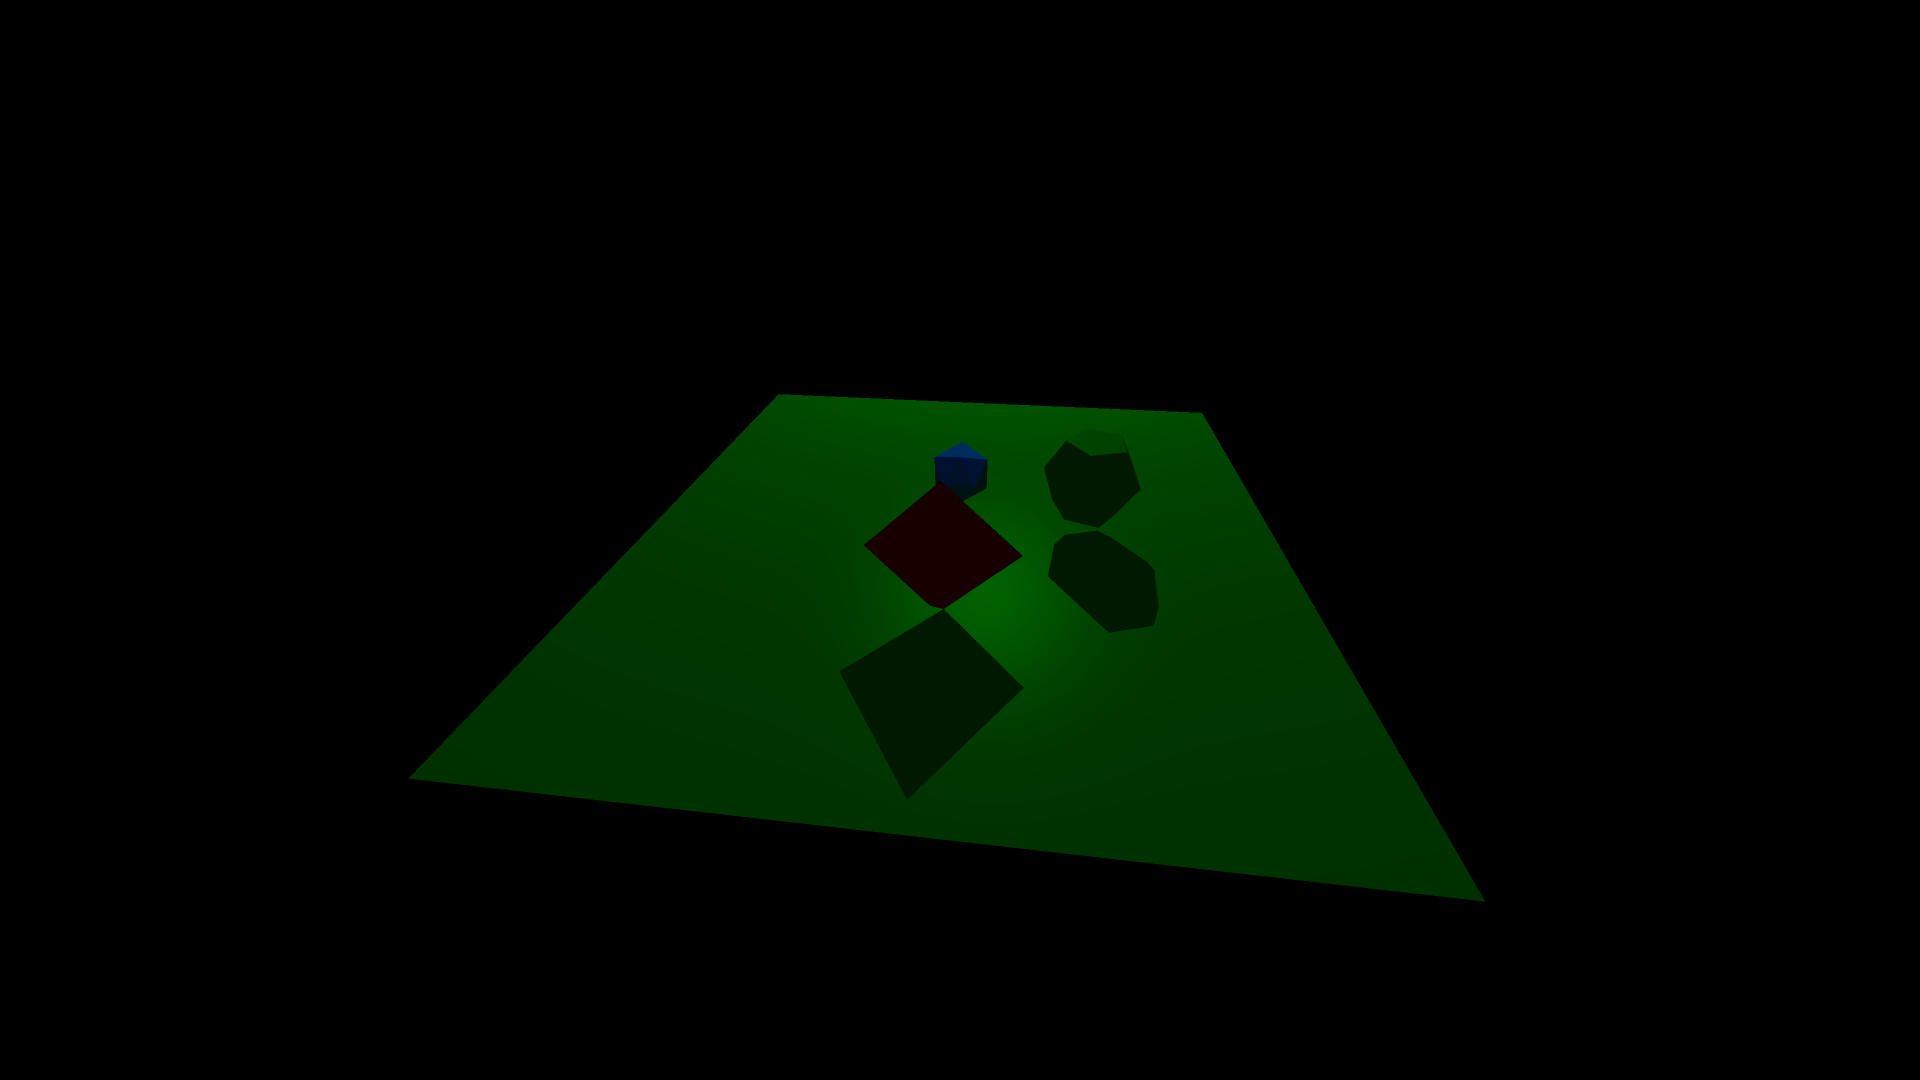
\includegraphics[scale=0.20]{11.data.png}

\se{Выводы}

\end{document}
